% Two nuts and a 15-storey house — Combinatorics 20 of the abacus.
%
% Wordless on purpose (floor numbers are digits), so it builds once for both
% languages. Same rules as the other drawings: strokes black — rewritten to
% currentColor — fills mid-tone, no transparency.
\documentclass[tikz,dvisvgm,border=3pt]{standalone}

\definecolor{wall}{HTML}{9AA3AE}
\definecolor{window}{HTML}{5E6874}
\definecolor{roof}{HTML}{6E7885}
\definecolor{nut}{HTML}{9A6B3A}
\definecolor{nutdark}{HTML}{744E27}
\definecolor{soil}{HTML}{A89377}

\begin{document}
% 1 unit of y = one storey.
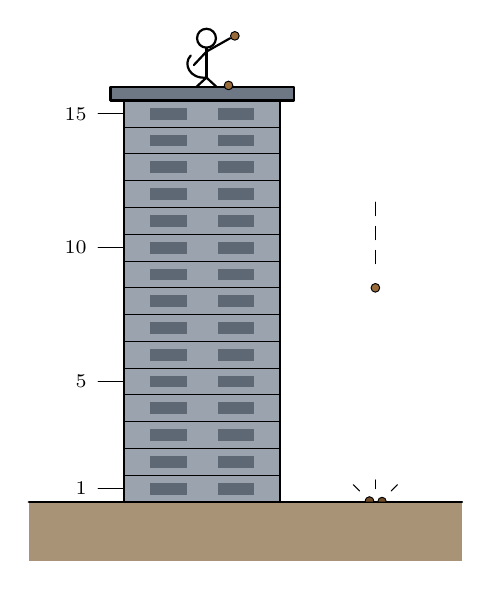
\begin{tikzpicture}[
  x=1.1cm, y=0.34cm,
  line join=round, line cap=round,
  edge/.style={line width=0.9pt},
  thin_/.style={line width=0.35pt},
  lbl/.style={font=\scriptsize},
]

% ── the ground ────────────────────────────────────────────────────────────
\fill[soil] (-1.1,0) rectangle (3.9,-2.2);
\draw[edge] (-1.1,0) -- (3.9,0);

% ── the house, fifteen storeys of it ──────────────────────────────────────
\fill[wall] (0,0) rectangle (1.8,15);
\draw[edge] (0,0) rectangle (1.8,15);
\foreach \i in {1,...,14} { \draw[thin_] (0,\i) -- (1.8,\i); }
\foreach \i in {0,...,14} {
  \fill[window] (0.3,\i+0.28) rectangle (0.72,\i+0.72);
  \fill[window] (1.08,\i+0.28) rectangle (1.5,\i+0.72);
}
\fill[roof] (-0.16,15) rectangle (1.96,15.5);
\draw[edge] (-0.16,15) rectangle (1.96,15.5);

% every fifth storey is numbered, on the left
\foreach \i in {5,10,15} {
  \draw[thin_] (-0.3,\i-0.5) -- (0,\i-0.5);
  \node[lbl, anchor=east] at (-0.32,\i-0.5) {\i};
}
\node[lbl, anchor=east] at (-0.32,0.5) {1};
\draw[thin_] (-0.3,0.5) -- (0,0.5);

% ── the monkey on the roof, one nut in hand and one at her feet ───────────
\begin{scope}[shift={(0.95,15.5)}, x=1cm, y=1cm, line width=0.8pt]
  \draw (0,0.12) -- (0,0.5);                      % body
  \fill[white] (0,0.62) circle (0.12);
  \draw (0,0.62) circle (0.12);                   % head
  \draw (0,0.45) -- (0.3,0.62);                   % the arm holding a nut out
  \draw (0,0.45) -- (-0.16,0.28);
  \draw (0,0.12) -- (-0.13,0);                    % legs
  \draw (0,0.12) -- (0.13,0);
  \draw (0,0.12) .. controls (-0.22,0.1) and (-0.3,0.3) .. (-0.2,0.4); % tail
  \fill[nut] (0.36,0.65) circle (0.055);          % the nut in hand
  \draw[line width=0.35pt] (0.36,0.65) circle (0.055);
  \fill[nut] (0.28,0.02) circle (0.055);          % the spare one
  \draw[line width=0.35pt] (0.28,0.02) circle (0.055);
\end{scope}

% ── one nut on its way down ───────────────────────────────────────────────
\fill[nut] (2.9,8) circle (0.055cm);
\draw[thin_] (2.9,8) circle (0.055cm);
\foreach \i in {1,2,3} { \draw[thin_] (2.9,8+0.9*\i) -- (2.9,8+0.9*\i+0.5); }

% ── and one that did not survive the trip ─────────────────────────────────
\begin{scope}[shift={(2.9,0)}, x=1cm, y=1cm]
  \fill[nutdark] (-0.13,0) .. controls (-0.13,0.09) and (-0.02,0.09) .. (-0.02,0) -- cycle;
  \draw[thin_] (-0.13,0) .. controls (-0.13,0.09) and (-0.02,0.09) .. (-0.02,0) -- cycle;
  \fill[nutdark] (0.03,0) .. controls (0.03,0.08) and (0.14,0.08) .. (0.14,0) -- cycle;
  \draw[thin_] (0.03,0) .. controls (0.03,0.08) and (0.14,0.08) .. (0.14,0) -- cycle;
  \draw[thin_] (-0.2,0.14) -- (-0.28,0.22);
  \draw[thin_] (0.2,0.14) -- (0.28,0.22);
  \draw[thin_] (0,0.17) -- (0,0.28);
\end{scope}

\end{tikzpicture}
\end{document}
